\section{Behavior of non-linear systems}
\label{nlinHamiltonian:section}

\LAtt{8.2}

\LO{
\item Find the trajectories for a non-linear system,
\item Determine if a system is Hamiltonian and use that fact to find the general solution, 
\item Use nullclines to help analyze a non-linear system, and
\item Identify basins of attraction and separatrices for a non-linear system.
}

\subsection{Conservative equations}

An equation of the form
\begin{equation*}
x'' + f(x) = 0
\end{equation*}
for an arbitrary function $f(x)$ is called a
\emph{\myindex{conservative equation}}.  For example the pendulum equation
is a conservative equation.  The equations are conservative as there is no
friction in the system so the energy in the system is \myquote{conserved.}
Let us write this equation as a
system of nonlinear ODE.
\begin{equation*}
x' = y, \qquad y' = -f(x) .
\end{equation*}
These types of equations have the
advantage that we can solve for their trajectories easily.

\begin{definition}
Assume that we have an autonomous system of differential equations defining $x$ and $y$, 
\begin{equation*}
x' = f(x,y) \qquad y' = g(x,y).
\end{equation*}
A \emph{\myindex{trajectory}} for this system is a curve in the $xy$-plane that the solution curve $(x(t), y(t))$ will stay on for all $t$. This curve will generally be given with $y$ as a function of $x$, or the level curve of some function $F(x,y)$. 
\end{definition}

For conservative equations, we want to first think of $y$ as a function of $x$ for a moment.  Then
use the chain rule
\begin{equation*}
x'' = y' = \frac{dy}{dx} x' = y \frac{dy}{dx} ,
\end{equation*}
where the prime indicates a derivative with respect to $t$.  
We obtain $y \frac{dy}{dx} + f(x) = 0$.  We integrate with respect to
$x$ to get
$\int y \frac{dy}{dx} \,dx + \int f(x)\, dx = C$.  In other words
\begin{equation*}
\frac{1}{2} y^2  + \int f(x)\, dx = C .
\end{equation*}
We obtained an implicit equation for the trajectories, with different $C$
giving different trajectories.  The value of
$C$ is conserved on any trajectory.  This expression is
sometimes called the \emph{\myindex{Hamiltonian}} or the energy of the
system.
If you look back to \sectionref{exact:section}, you will notice
that $y\frac{dy}{dx} + f(x) = 0$ is an exact equation, and
we just found a potential function.

Another approach we could use in this case is separable equations, if it works out. The idea is that we have the system
\begin{equation*}
x' = y, \qquad y' = -f(x)
\end{equation*}
and want to develop a differential equation for $y$ in terms of $x$. We can write this differential equation using some principles from implicit differentiation and parametric equations as
\begin{equation*}
\frac{dy}{dx} = \frac{dy/dt}{dx/dt},
\end{equation*}
which, for this case, is 
\begin{equation*}
\frac{dy}{dx} = \frac{-f(x)}{y}.
\end{equation*}
This equation is separable as
\begin{equation*}
y\ dy = -f(x)\ dx
\end{equation*}
and we can get to the same implicit equation for the trajectories as before. 

\begin{example}
Find the trajectories for the equation $x'' + x-x^2 = 0$,
which is the equation from
\examplevref{example:nlin-1b-example}.
\end{example}

\begin{exampleSol}  
The corresponding
first order system is
\begin{equation*}
x' = y , \qquad y' = -x+x^2 .
\end{equation*}
Trajectories satisfy
\begin{equation*}
\frac{1}{2} y^2  + \frac{1}{2} x^2 - \frac{1}{3} x^3  = C .
\end{equation*}
We solve for $y$
\begin{equation*}
y = \pm \sqrt{-x^2 + \frac{2}{3} x^3  + 2C} .
\end{equation*}

Plotting these graphs we get exactly the trajectories in 
\figurevref{fig:nlin-1b}.  In particular we notice that near the origin
the trajectories are \emph{\myindex{closed curves}}: they keep going
around the origin, never spiraling in or out.  Therefore we discovered a way
to verify that the critical point at $(0,0)$ is a stable center.
The critical point at $(0,1)$ is a saddle as we already noticed.
This example is typical for conservative equations.
\end{exampleSol}

Consider an arbitrary
conservative equation $x'' + f(x) = 0$.
All critical points occur when $y=0$ (the
$x$-axis), that is when $x' = 0$.  The critical points are 
those points on the $x$-axis where $f(x) = 0$.
The trajectories are given by
\begin{equation*}
y = \pm \sqrt{ - 2 \int f(x)\, dx + 2C} .
\end{equation*}
So all trajectories are mirrored across the $x$-axis.  In particular,
there can be no spiral sources nor sinks.
The Jacobian matrix is
\begin{equation*}
\begin{bmatrix}
0 & 1 \\
-f'(x) & 0
\end{bmatrix} .
\end{equation*}
The critical point is almost linear if $f'(x) \not= 0$ at the critical 
point.  Let $J$ denote the Jacobian matrix.
The eigenvalues of $J$ are solutions to
\begin{equation*}
0 = \det(J - \lambda I) = \lambda^2 + f'(x) .
\end{equation*}
Therefore $\lambda = \pm \sqrt{-f'(x)}$.  In other words, either we get
real eigenvalues of opposite signs (if $f'(x) < 0$),
or we get purely imaginary eigenvalues (if $f'(x) > 0$).
There are only two possibilities for critical points, either an \emph{unstable
saddle point}, or a \emph{stable center}.
There are never any sinks or sources.

\subsection{Hamiltonian Systems}

A generalization of conservative equations to systems is a \myindex{Hamiltonian} system. This type of system has all of the nice properties of conservative equations when converted into systems, but allows for more general interactions between $x$ and $y$. For these systems, the point is that the equation has a conserved quantity called a Hamiltonian, which does not change as the system evolves in time, which generally represents the energy of the system. Calling this function $H(x,y)$, this means that
\[ \frac{d}{dt}H(x,y) = 0. \] By the chain rule, this is equivalent to
\[ \frac{\partial H}{\partial x} \frac{dx}{dt} + \frac{\partial H}{\partial y} \frac{dy}{dt} = 0.\]

One way to satisfy this is with 
\begin{equation}
\begin{split}
\frac{dx}{dt} &= -\frac{\partial H}{\partial y} \\
\frac{dy}{dt} &= \frac{\partial H}{\partial x}
\end{split}
\label{eq:HamilDef}
\end{equation} 

and this gives the definition of a \emph{Hamiltonian system}. 

\begin{definition}
The system
\begin{equation}
\begin{split}
\frac{dx}{dt} &=f(x,y) \\
\frac{dy}{dt} &= g(x,y)
\end{split}
\end{equation} 
is \emph{Hamiltonian} if there is a function $H(x,y)$ so that $f(x,y) = -\frac{\partial H}{\partial y}$ and $g(x,y) = \frac{\partial H}{\partial x}$. 
\end{definition}

For solving these sorts of systems, we know that 
\[ \frac{d}{dt}H(x,y) = 0, \]
since that's how we defined the system. This means that the trajectories of this system are given by
\[ H(x,y) = C \] for a constant $C$ determined by initial conditions. So if we can find the function $H$ that expresses the system in the form \eqref{eq:HamilDef}, then we are done.

Finding this $H$ is a lot similar to finding solutions to exact equations in \sectionref{exact:section}. First, we need to determine if the system is Hamiltonian. Since we want to have that
\[ f(x,y) = -\frac{\partial H}{\partial y} \qquad g(x,y) = \frac{\partial H}{\partial x} \]
we know that
\[ f_x(x,y) = -\frac{\partial^2 H}{\partial x \partial y} \qquad g_y(x,y) = \frac{\partial^2 H}{\partial x \partial y} \] which shows that
\[ f_x + g_y = 0. \] This is what we can use to check if a system is Hamiltonian; compare to Theorem \ref{thm:Poincare} for exact equations.

Once we know that a system is Hamiltonian, we can integrate the different components of the equation to find the function $H$. Since $f = -\frac{\partial H}{\partial y}$, then we can write
\[ H(x,y) = -\int f(x,y)\ dy + A(x) \] where $A(x)$ is an unknown function, which can be determined by differentiating this in $x$ and setting equal to $g(x,y)$.

\begin{example}
Consider the system of differential equations given by
\[ x' = -4x + 3y \qquad y' = 2x + 4y. \]
Determine if this system is Hamiltonian and, if so, find the trajectories of the solution.
\end{example}

\begin{exampleSol}
We first check if $f_x + g_y = 0$ to see if the system is Hamiltonian. Since $f_x = -4$ and $g_y = 4$, this means we have a Hamiltonian system. In order to find the function $H$, we use that
\[ \frac{\partial H}{\partial y} = -f(x,y) = 4x - 3y. \]
Integrating both sides in $y$ gives that
\[ H(x,y) = 4xy - \frac{3}{2}y^2 + A(x) \] for an unknown function $A(x)$. Differentiating this in $x$ gives 
\[ \frac{\partial H}{\partial x} = 4y + A'(x) \] which we want to equal $2x + 4y$. This gives that $A'(x) = 2x$ so $A(x) = x^2$. Thus, the Hamiltonian is given by
\[ H(x,y) = x^2 + 4xy - \frac{3}{2}y^2 \] so that the trajectories are defined by 
\[ x^2 + 4xy - \frac{3}{2}y^2 = C\] for any constant $C$. These are sketched in \figureref{fig:HamilPlot}.

\begin{myfig}
\capstart
\myincludegraphics{width=3in}{width=4.5in}{HamilPlot}
\caption{Vector field and trajectories for a Hamiltonian System \label{fig:HamilPlot}}
\end{myfig}

Note that this system is linear and autonomous. Therefore, we could have solved this using those methods as well. For this, we have the coefficient matrix 
\begin{equation*}
A = \begin{bmatrix} 
-4 & 3 \\ 2 & 4 \end{bmatrix}
\end{equation*}
and we can find the eigenvalues of this matrix as the roots of
\begin{equation*}
\det(A - \lambda I) = (-4-\lambda)(4-\lambda) - (3)(2)  = \lambda^2 - 22
\end{equation*}
whose roots are $\pm\sqrt{22}$ which have opposite signs. Therefore, this will be a saddle point, which we see represented in the plot in \figureref{fig:HamilPlot}.
\end{exampleSol}


\subsection{Separatrices and Basins of Attractions}

If we have an asymptotically stable critical point $(x_0, y_0)$ for an autonomous system of differential equation, we know that solutions that start ``near'' this point will converge to it as $t \rightarrow \infty$. That's what it means for the point to be asymptotically stable. However, for applications, it may be important to know exactly which initial conditions $(x(0), y(0))$ will end up converging to $(x_0, y_0)$. This can be particularly relevant when there are multiple asymptotically stable equilibrium solutions and we need to determine which one a given initial condition will converge to. 

\begin{definition}[Basin of attraction]
Let $(x_0, y_0)$ be an asymptotically stable equilibrium solution for the autonomous system $\vec{x}\ ` = \vec{F}(x,y)$. The \emph{\myindex{basin of attraction}} for $(x_0, y_0)$ is the set of all points $(a,b)$ where the solution to
\begin{equation*}
\vec{x}' = \vec{F}(x,y) \qquad \vec{x}(0) = \begin{bmatrix} a \\ b \end{bmatrix}
\end{equation*}
converges to $(x_0, y_0)$ as $t \rightarrow \infty$.
\end{definition}

In general, the basin of attraction for an asymptotically stable critical point is difficult, if not impossible, to find analytically. The main approach here is to use a direction field to approximate the basin of attraction.

\begin{example} \label{ex:BoA}
Find all asymptotically stable critical points for the autonomous system
\begin{equation*}
\frac{dx}{dt} = x(7-2x-5y) \qquad \frac{dy}{dt} =(y+1)(5-3x-2y)
\end{equation*}
and determine an approximate basin of attraction for each. 
\end{example}

\begin{exampleSol}
We want to start by finding the critical points for this system, classifying them to determine if they are asymptotically stable, and then use a slope field to try to find the basin of attraction. In order to have a critical point, we need to have both $\frac{dx}{dt}$ and $\frac{dy}{dt}$ equal to zero. This means that we need
\begin{equation*}
\left[ x=0 \text{ or } 7-2x-5y = 0\right] \quad \text{ and } \quad \left[ y=-1 \text{ or } 5 - 3x - 2y = 0 \right]. 
\end{equation*}
This results in the points $(0, -1)$, $\left(0, \nicefrac{5}{2}\right)$, $(6, -1)$, and $(1, 1)$. In order to classify each of these critical points, we need to find the Jacobian matrix for this system, which is
\begin{equation*}
J(x,y) = \begin{bmatrix} F_x & F_y \\ G_x & G_y \end{bmatrix} = \begin{bmatrix} 7-4x-5y & -5x \\ -3(y+1) & 3 - 3x - 4y \end{bmatrix},
\end{equation*}
and then we want to plug each critical point into this matrix in turn. 

Plugging in $(0,-1)$ gives $\left[ \begin{smallmatrix} 12 & 0 \\ 0 & 7 \end{smallmatrix} \right]$, which has eigenvalues of $12$ and $7$, and so is a nodal source, which is unstable. Plugging in  $\left(0, \nicefrac{5}{2}\right)$ gives $\left[ \begin{smallmatrix} -\nicefrac{11}{2} & 0 \\ -\nicefrac{21}{2} & -7 \end{smallmatrix} \right]$, which has eigenvalues of $-\nicefrac{11}{2}$ and $-7$, which is a nodal sink, and so asymptotically stable. Plugging in $(6,-1)$ gives $\left[ \begin{smallmatrix} -12 & 30 \\ 0 & -11 \end{smallmatrix} \right]$, which has eigenvalues at $-11$ and $-12$, giving an asymptotically stable nodal sink. The last point at $(1,1)$ gives $\left[ \begin{smallmatrix} -2 & -5 \\ -6 & -4 \end{smallmatrix} \right]$, which is not triangular, and so does not have easily identifiable eigenvalues. We could use trace-determinant analysis to classify (\sectionref{sec:twodimaut}) or we can just compute the eigenvalues. Those are found by the roots of
\begin{equation*}
\det(A - \lambda I) = (-2-\lambda)(-4-\lambda) - (-5)(-2) = \lambda^2 + 6\lambda - 2
\end{equation*}
and since the last term is negative, we know we are going to get roots of opposite signs, so this is an unstable saddle point. The actual eigenvalues are
\begin{equation*}
\frac{-6 \pm \sqrt{36 - 4(1)(-2)}}{2} = -3 \pm \frac{\sqrt{44}}{2} = -3\pm\sqrt{11}.
\end{equation*}

So, this means we have two asymptotically stable critical points, $\left(0, \nicefrac{5}{2}\right)$ and $(6, -1)$. We need to look at a slope field to determine the approximate basin of attraction for each of these points.

\begin{myfig}
\capstart
\myincludegraphics{width=6in}{width=7in}{BoASlopeEx1}
\caption{Plots showing the slope field for \exampleref{ex:BoA} (left) and a slope field combined with approximate basins of attraction (right). \label{fig:BoAPlot}}
\end{myfig}

From \figureref{fig:BoAPlot}, we can see that there is a sort of dividing line between the two nodal sinks. If the solution starts on one side of the line, it funnels into one critical point, and on the other side, it heads to the other one. This dividing line also seems to pass through the saddle point at $(1,1)$, which is not a coincidence, as we will see later. 
\end{exampleSol}

Another interesting feature of these regions is the boundary of them. This is a curve that separates solutions that converge to the asymptotically stable equilibrium solution and those that don't. This leads to another definition.

\begin{definition}[Separatrix]
Consider the autonomous system $\vec{x}' = \vec{F}(x,y)$. A \emph{\myindex{separatrix}} (plural separatrices) is a curve in the plane that separates trajectories that have different long-term behaviors of solutions to $\vec{x}\ ` = \vec{F}(x,y)$.
\end{definition}

The boundary of a basin of attraction is a separatrix because the long-term behavior inside the curve (converging to the asymptotically stable critical point) is different from the behavior outside the curve (going somewhere else). These dividing curves also show up in other contexts.

\begin{example} \label{ex:Separatrix}
Analyze the system
\begin{equation*}
\begin{split}
\frac{dx}{dt} &= -x -y\\
\frac{dy}{dt} &= -2x
\end{split}
\end{equation*}
in the context of separatrices.
\end{example}

\begin{exampleSol}
This is a linear, homogeneous system, so we can analyze it via that approach. For the coefficient matrix $A = \left[ \begin{smallmatrix} -1 & -1 \\ -2 & 0 \end{smallmatrix} \right]$, we have eigenvalues as the roots of $(-1-\lambda)(-\lambda) - 2$, or $\lambda^2 + \lambda - 2$. Therefore, the eigenvalues here are $1$ and $-2$. For $1$ we have eigenvector $\left[ \begin{smallmatrix} 1 \\ -2 \end{smallmatrix}\right]$ and for $-2$, an eigenvector is $\left[ \begin{smallmatrix} 1 \\ 1 \end{smallmatrix}\right]$. We can see what this looks like on a slope field in \figureref{fig:SepPlot}.


\begin{mywrapfig}{3.3in}
\capstart
\myincludegraphics{width=3in}{width=4in}{SaddleSeparatrix}
\caption{Plot showing the slope field for \exampleref{ex:Separatrix} with a sketch of the separatrix. \label{fig:SepPlot}}
\end{mywrapfig}

There are no asymptotically stable critical points here, so there are no basins of attraction. However, there are two distinct behaviors of the solution curve. It is going away from the origin, but it could go to the top left, or to the bottom right. Both of those make sense based on the slope field here. So how do we know which way it goes? The line drawn on the right side of \figureref{fig:SepPlot} seems to divide these two regions up. If the solution starts above the line, it goes to the top left, otherwise, it goes to the bottom right. This is the separatrix for this saddle point.

But what is that line? If we inspect the graph more closely, the separatrix here is the straight-line solution that converges to zero over time; the one particular solution that does not go off to infinity because it only has the $e^{-2t}$ term in it. So the straight-line solutions that flow into saddle points divide what happens on the two sides of it. This is a very common fact in looking at separatrices: if they go through a critical point, they generally do so as the in-flowing solution from a saddle point. All of the examples we have seen so far with separatrices have done exactly this.
\end{exampleSol}

\subsection{Nullclines}

When trying to find critical points for a non-linear, autonomous system, we need all (both, in the case of two component systems) of the equations to be zero. What happens if only one of the equations is zero? This is a lot easier to find, and can also give us a fair bit of information. 

\begin{definition}[Nullcline] 
Consider the autonomous two-component system
\begin{equation*}
\frac{dx}{dt} = f(x,y) \qquad \frac{dy}{dt} = g(x,y).
\end{equation*}
A \emph{\myindex{nullcline}} for this system is a curve where either $f(x,y) = 0$ or $g(x,y) = 0$. We can also be more specific and use the term \emph{x-nullcline} for the curve(s) where $\frac{dx}{dt} = 0$ and \emph{y-nullcline} for where $\frac{dy}{dt} = 0$.
\end{definition}

The way we can use these nullclines is to know in general which direction the solution curve will move in different regions of the plane. Assuming that all of the functions involved are continuous, if we know that the solution at a given point will move to the right, that is, if $\frac{dx}{dt} > 0$, then we know that the solution will continue to move to the right until we cross an $x$-nullcline. If the solution starts going back to the left, this means that $\frac{dx}{dt}$ becomes negative, and so must cross zero, which is where a nullcline is.

In addition, we know that along an $x$-nullcline, $\frac{dx}{dt} = 0$, so the solution can only be moving in the $y$ direction, that is, vertically. If we can determine in which direction the solution graph will cross the nullclines, this can also be helpful and useful. It doesn't give as much information as a full slope field or trajectory plot, but it can give a general idea of what is going to happen to the solution over time. 

\begin{example} \label{ex:Nullcline1}
Use a nullcline analysis to determine the overall behavior of solutions to the system
\begin{equation*}
\frac{dx}{dt} = (y-1)(x-y) \qquad \frac{dy}{dt} = (x+3)(x-2).
\end{equation*}
\end{example}

\begin{exampleSol}
We can get the equations for nullclines from the factors of each of the differential equations here. For $x$-nullclines, we get $y=1$ and $y=x$, and for $y$-nullclines, we get $x=-3$ and $x=2$. Once we have these lines, we need to determine what happens within each of the regions on the resulting graph. For example, if we look in the region above $y=1$, above $y=x$ and right of $x=2$, we can plug in, for example $(3,4)$. At this point $\frac{dx}{dt} = (4-1)(3-4) = -3 < 0$ and $\frac{dy}{dt} = (3+3)(3-2) = 6 > 0$. Therefore, the solution here moves up and to the left. We can fill in all of the other regions in a similar manner. This is shown on the left of \figureref{fig:NCPlot1}.

\begin{myfig}
\capstart
\myincludegraphics{width=5in}{width=6.5in}{NCSlopeEx1}
\caption{Plots showing the nullcline diagram for \exampleref{ex:Nullcline1} (left) and a slope field for the same differential equation (right). \label{fig:NCPlot1}}
\end{myfig}

Based on the nullcline diagram here, we can see that there seems to be some sort of spiraling behavior around both $(2,2)$ and $(-3, -3)$, which we know are critical points because the two different nullclines intersect there. From this alone, we can't really tell if they are sources, sinks, or centers, but we do get a general idea of the behavior. We also see what looks like saddles at $(-3, 1)$ and $(2, 1)$, since these critical points have two opposite arrows pointing towards this point (corresponding to the negative eigenvalue of the linearized system), and two opposite arrows pointing away from the point (corresponding to the positive eigenvalue. The slope field seems to validate all of these general discussions from the nullcline diagram.
\end{exampleSol}



\begin{example} \label{ex:Nullcline2}
Use a nullcline analysis to determine the overall behavior of solutions to the system
\begin{equation*}
\frac{dx}{dt} = (x-3)(y+1) \qquad \frac{dy}{dt} = (y-2)(x+y).
\end{equation*}
\end{example}

\begin{exampleSol}
As with the previous example, we can find the nullcline equations from the factors above. The $x$-nullclines are at $x=3$ and $y=-1$, and the $y$-nullclines are at $y=2$ and $x=-y$. We can plug in points to fill in the nullcline diagram like before, and compare to the slope field, shown in \figureref{fig:NCPlot2}. 

\begin{myfig}
\capstart
\myincludegraphics{width=5in}{width=6.5in}{NCSlopeEx2}
\caption{Plots showing the nullcline diagram for \exampleref{ex:Nullcline2} (left) and a slope field for the same differential equation (right). \label{fig:NCPlot2}}
\end{myfig}

In this diagram, we see some of the other types of critical points and what they look like through nullclines. The point at $(3,2)$ looks like a nodal source, because all of the arrows point away from that point, and $(3,-3)$ looks like a nodal source. Finally, we see a potential saddle at $(1,-1)$ because of the patterns of the arrows, all of which are also shown in the slope field for this system.

An extra point with this type of result is that we know we can not cross the nullclines at $x=3$ and $y=2$. For instance, the line $x=3$ is an $x$-nullcline. This means that the solution must cross the line moving vertically. However, it is a vertical line, and there is no way to cross a vertical line moving vertically. The same argument applies to $y=2$. We can also see this by the fact that the arrows on either side of the line both point into or away from these nullclines.
\end{exampleSol}


\subsection{Exercises}


\begin{exercise}
\pagebreak[2]
Find the implicit equations of the trajectories of the following
conservative systems.  Next find their critical points (if any) and classify them.
\begin{tasks}(2)
\task $x''+ x+x^3 = 0$
\task $\theta''+\sin \theta = 0$
\task $z''+ (z-1)(z+1) = 0$
\task $x''+ x^2+1 = 0$
\end{tasks}
\end{exercise}

\begin{exercise}\ansMark%
Find the implicit equations of the trajectories of the following
conservative systems.  Next find their critical points (if any) and classify them.
\begin{tasks}(3)
\task $x''+ x^2 = 4$
\task $x''+ e^x = 0$
\task $x''+ (x+1)e^x = 0$
\end{tasks}
\end{exercise}
\exsol{%
a) $\frac{1}{2}y^2 + \frac{1}{3}x^3 -4x = C$, critical points:
$(-2,0)$, an unstable saddle, and $(2,0)$, a stable center. \quad
b) $\frac{1}{2}y^2 + e^x = C$, no critical points. \quad
c) $\frac{1}{2}y^2 + xe^x = C$, critical point at $(-1,0)$ is a stable center.
}


\begin{exercise}\ansMark%
The conservative system $x''+x^3 = 0$ is not almost linear.  Classify
its critical point(s) nonetheless.
\end{exercise}
\exsol{%
Critical point at $(0,0)$.
Trajectories are $y = \pm \sqrt{2C-(\nicefrac{1}{2})x^4}$, for $C > 0$, these give closed
curves around the origin, so the critical point is a stable center.
}

\begin{exercise}
Determine if the following system is Hamiltonian. If it is, find the general solution in the form $H(x,y) = C$ and sketch some of the trajectories.
\[ \frac{dx}{dt} = x - 2y \qquad \frac{dy}{dt} = 3x - y.\]
\end{exercise}

\begin{exercise}
Determine if the following system is Hamiltonian. If it is, find the general solution in the form $H(x,y) = C$ and sketch some of the trajectories.
\[ \frac{dx}{dt} = 4x - 2y + 2 \qquad \frac{dy}{dt} = -5x + y - 1.\]
\end{exercise}


\begin{exercise}
Determine if the following system is Hamiltonian. If it is, find the general solution in the form $H(x,y) = C$ and sketch some of the trajectories.
\[ \frac{dx}{dt} = x^2 - 2xy + 3y^2 \qquad \frac{dy}{dt} = y^2 - 2xy + e^x .\]
\end{exercise}


\begin{exercise}
Determine if the following system is Hamiltonian. If it is, find the general solution in the form $H(x,y) = C$ and sketch some of the trajectories.
\[ \frac{dx}{dt} = 3x - 2xy \qquad \frac{dy}{dt} = 2xy - 3y.\]
\end{exercise}

\begin{exercise} Consider a generic thing on a spring, with displacement $u$ and velocity $v$. Assume that $$mu''+ku=0,$$ where $m$ and $k$ are some positive constants.
\begin{tasks}
\task Rewrite this equation as a {\it first-order} system in $u$ and $v$.
\task Find a Hamiltonian function for this system (in terms of $u$ and $v$).
\task What shapes are the level curves of the Hamiltonian function? 
\task Does this system have a {\it basin of attraction}? Explain briefly. 
\end{tasks}
\end{exercise}

\begin{exercise}
Suppose $f$ is always positive.
Find the trajectories of $x''+f(x') = 0$.
Are there any critical points?
\end{exercise}

\begin{exercise}
Suppose that $x' = f(x,y)$, $y' = g(x,y)$.  Suppose that $g(x,y) > 1$ for
all $x$ and $y$.  Are there any critical points?  What can we say about the
trajectories at $t$ goes to infinity?
\end{exercise}

\begin{exercise}
Here is the direction field for the system $\dfrac{dx}{dt}=y^2-3y, \dfrac{dy}{dt}=x^2-4x$. The critical points are $(0,0), (4,0), (0,3)$, and $(4,3)$. Draw the nullclines on the plot. What do the nullclines tell us about the critical points?

\begin{center}
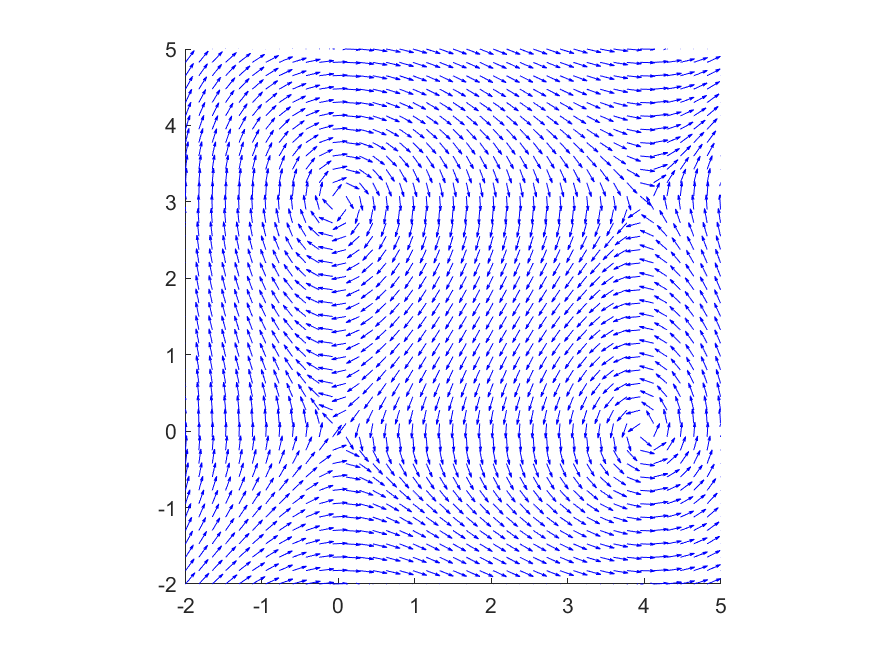
\includegraphics[width=0.6\textwidth]{Images/NLVF_1.png}
\end{center}
\end{exercise}

\begin{exercise}
Nullclines apply to linear systems as well, although since we can often solve those explicitly they're less necessary. Construct the nullcline diagram for the system $\dfrac{dx}{dt}=-3x+y$, $\dfrac{dy}{dt}=6x+2y$, and use it to classify (by type) the equilibrium point at the origin. What is the {\it linearization} of this system at $(0,0)$?
\end{exercise}

\begin{exercise}
Consider the system $\displaystyle \frac{dx}{dt}= -2x+y, \frac{dy}{dt}=-y+x^2$.
\begin{tasks}
\task Find all equilibrium solutions.
\task Sketch all nullclines for this system on a single diagram. Label each region, and use these results to classify each equilibrium point.
\end{tasks}
\end{exercise}

\begin{exercise} Nullclines need not be lines. Consider the system
$$\begin{bmatrix} \displaystyle \frac{dx}{dt}=4-y^2\\ \dfrac{dy}{dt}=8-x^2-y^2 \end{bmatrix}.$$

\begin{tasks}
\task Find all critical points of this system.
\task Sketch the nullcline diagram and label all regions DL, DR, UL, or UR. Classify (according to type) any critical point(s) that can be classified using this analysis.
\task Two critical points cannot be classified using the nullcline analysis. Classify these (again according to type) using the Jacobian. 
\end{tasks}
\end{exercise}

\begin{exercise}
Consider the system
\begin{equation}
\begin{bmatrix}
\frac{dx}{dt}=x-y^2+2\\[12pt]
\frac{dy}{dt}=x^2-y^2
 \end{bmatrix}
\label{eq:CriticalHamilEx}
\end{equation}
%5.1
\begin{tasks}
\task Find all critical points of \eqref{eq:CriticalHamilEx}.
\task Create the nullcline diagram for the system, labelling each region as one of UL, UR, DL, or DR. Use this information to classify two critical points according to type.
\task Use the Jacobian matrix to classify any remaining critical points.
\task Is there a conserved quantity (Hamiltonian function) for this system? If so, find one. If not, explain why not.
\end{tasks}
\end{exercise}

\begin{exercise}
 For a conflict between two armies, Lanchester's Law asserts that $\dfrac{dx}{dt}=-\alpha y$ and $\dfrac{dy}{dt}=-\beta x$, %5.2 (Hamiltonian, separatrix)
where $x$ and $y$ are the two populations, and $\alpha$ and $\beta$ are some positive constants.

\begin{tasks}
\task Find a Hamiltonian function for this system satisfying $H(0,0)=0$. 
\task Classify the critical point at the origin according to type {\bf and} stability.
\task Assume that we are just looking at the first quadrant, since the populations are non-negative. Find the curve along which the Hamiltonian function is zero, and explain its significance in terms of who wins the conflict.
\end{tasks}
\end{exercise}

\begin{exercise}
Consider the non-linear system
\begin{equation}
\frac{dx}{dt}=4x-3y-x(x^2+y^2), \ \frac{dy}{dt}=3x+4y-y(x^2+y^2). \label{eq:NonLinStabLimitEx1} %5.1 or 2
\end{equation}
\begin{tasks}
\task \eqref{eq:NonLinStabLimitEx1} has a critical point at the origin. What is the {\it linearization} of \eqref{eq:NonLinStabLimitEx1} at the origin?
\task Demonstrate that \eqref{eq:NonLinStabLimitEx1} is {\it locally linear} in a neighborhood of the origin. 
\task Classify the origin according to its {\it type} and {\it stability}.
\end{tasks}
\end{exercise}

\begin{exercise} 
Consider the system of differential equations
\begin{equation}
\frac{dx}{dt} = (x^2 - 1)y \qquad \frac{dy}{dt} = (y-3)(y-1)x \label{eq:NonLinBoAExam1}
\end{equation}
which has slope field sketched below.
\begin{center}
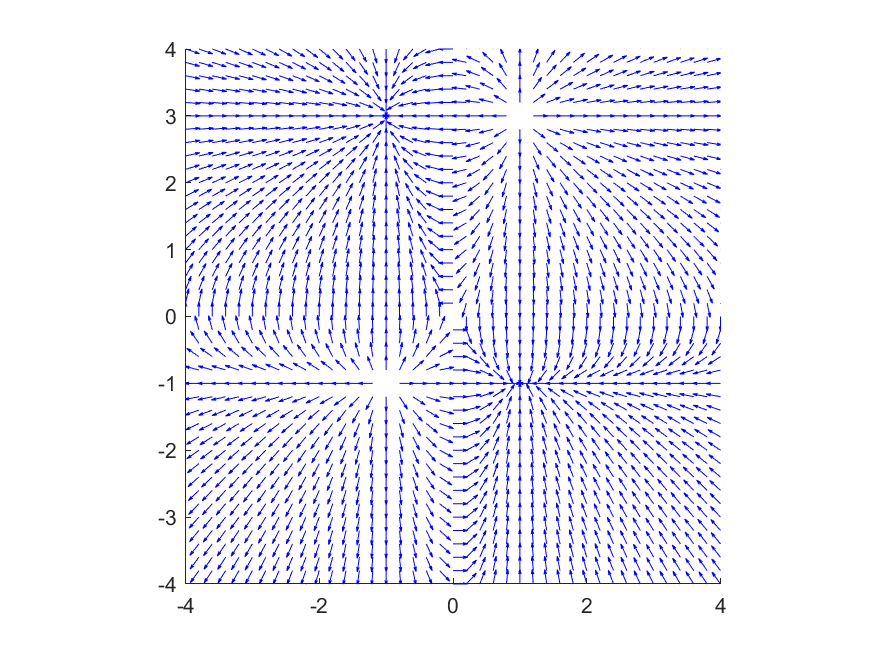
\includegraphics[width=0.6\textwidth]{Images/NLBoA_Ex1.png}
\end{center}
\begin{tasks}
\task Find and classify all critical points of the system \eqref{eq:NonLinBoAExam1}.
\task Draw any separatrices that you can spot on the slope field.
\task Do any of these critical points have a basin of attraction? If so, sketch out what regions of the plane correspond to a basin of attraction for those critical points. 
\end{tasks}
\end{exercise}

\begin{exercise} 
Consider the system of differential equations
\begin{equation}
\frac{dx}{dt} = (2-y)(y+1)(x+1) \qquad \frac{dy}{dt} = -(x+2)(x-1)y \label{eq:NonLinBoAExam2}
\end{equation}
which has slope field sketched below.
\begin{center}
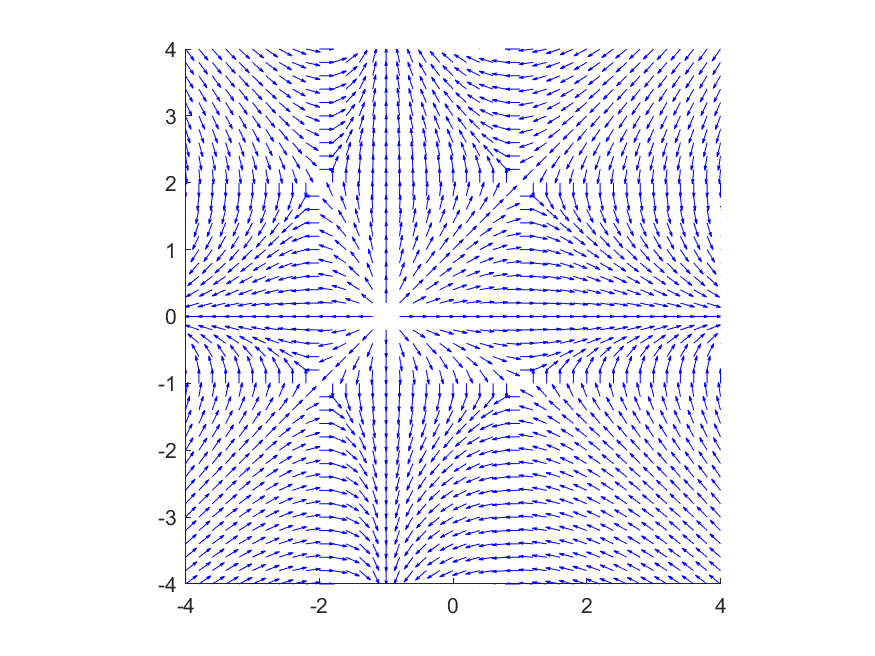
\includegraphics[width=0.6\textwidth]{Images/NLBoA_Ex2.png}
\end{center}
\begin{tasks}
\task Find and classify all critical points of the system \eqref{eq:NonLinBoAExam2}.
\task Draw any separatrices that you can spot on the slope field.
\task Do any of these critical points have a basin of attraction? If so, sketch out what regions of the plane correspond to a basin of attraction for those critical points. 
\end{tasks}
\end{exercise}

\setcounter{exercise}{100}
